\section{Hindcast Results}
	\subsection{Model Evaluation}
		Table \ref{tab:results-evaluation-inside-mm} shows the evaluation results for the three cities inside Metro Manila: Manila, Pasay, and Quezon.
		All MB and RMSE values fall within the recommended values of $\leq \pm \qty{2.0}{\degreeCelsius}$ and $\leq \qty{3.5}{\degreeCelsius}$, respectively.
		This shows that these simulations correctly follow the average air temperature for these respective cities.
		Despite this, many runs show an IOA value $< 0.8$, indicating that these runs show bad agreement between the simulation and observed data.
		While these runs may follow the average trend for air temperature in these cities, it may not be capturing the details of how the temperature changes.
		
		\begin{table}[]
			\caption{Evaluation results for the three cities inside Metro Manila. Values that do not match the recommended values are colored in red.}
			\label{tab:results-evaluation-inside-mm}
			\centering
			\begin{tabular}{lrSSSS}
				\hline \hline
				ICBC     & \multicolumn{1}{c}{ds [\unit{km}]} & {MB [\unit{\degreeCelsius}]} & {MAE [\unit{\degreeCelsius}]}                          & {RMSE [\unit{\degreeCelsius}]} & {IOA}                               \\
				\hline
				\multicolumn{6}{c}{\textit{Manila}}                                                                                                  \\
				EIN15    & 16                          & -0.53   & 1.27                              & 1.61      & \color{red} 0.78 \\
				EIN15    & 8                           & 0.90    & 1.45                              & 1.84      & 0.85                              \\
				CNRM-CM5 & 16                          & -0.73   & 1.63                              & 2.09      & \color{red}0.57 \\
				CNRM-CM5 & 8                           & -0.38   & 1.87                              & 2.33      & \color{red}0.75 \\
				\multicolumn{6}{c}{\textit{Pasay}}                                                               \\
				EIN15    & 16                          & -0.59   & 1.24                              & 1.55      & 0.88                              \\
				EIN15    & 8                           & 0.94    & 1.40                              & 1.75      & 0.88                              \\
				CNRM-CM5 & 16                          & -0.72   & 1.87                              & 2.39      & \color{red} 0.52 \\
				CNRM-CM5 & 8                           & -0.37   & 1.78                              & 2.22      & \color{red} 0.79 \\
				\multicolumn{6}{c}{\textit{Quezon}}                                                                                  \\
				EIN15    & 16                          & -0.61   & 1.45                              & 1.81      & 0.88                              \\
				EIN15    & 8                           & 0.57    & 1.33                              & 1.70      & 0.91                              \\
				CNRM-CM5 & 16                          & -0.10   & \color{red} 2.29 & 2.77      & \color{red} 0.46 \\
				CNRM-CM5 & 8                           & -0.75   & 1.95                              & 2.44      & 0.81  \\                           
				\hline
			\end{tabular}
		\end{table}
		
		For the MAE, the CNRM-CM5 run with 16 km horizontal resolution has a value of $2.29$ in Quezon, which does not fall within the recommended value of $\leq \pm \qty{2.0}{\degreeCelsius}$.
		All other MAE values for runs in Manila, Pasay, and Quezon fall within the recommended value.
		The same run also exhibits the lowest IOA value of $0.46$, indicating that this run exhibits the poorest agreement between the simulation and observed data.
		A graph of the simulation data and observed data for Quezon using CNRM-CM5 can be seen in Figure \ref{fig:cnrm-sim-vs-observed-quezon}. 
		The simulation with the lower grid cell resolution was able to follow the average trend of the observed data, but its oscillations were much smaller than the observed data.
		The simulation with the finer resolution matches the large oscillations of the observed data more closely (Figure 2b).
		This may indicate that the high MAE is due to the failure of that run to replicate the oscillations of the observed data.
		More graphs comparing the simulated and observed data for Manila, Quezon, and Pasay are found in Appendix \ref{app:model-evaluation-graphs}.

		
		\begin{figure}	
			\centering
			\includegraphics[width = \textwidth]{CNRM 16 km/Quezon}
			\includegraphics[width = \textwidth]{CNRM 8 km/Quezon}
			\caption{
				A comparison of the simulated data (orange) and observed data (blue) in the city of Quezon using the CNRM-CM5 ICBC with 16 km resolution (above) and 8 km resolution (below).
			}
			\label{fig:cnrm-sim-vs-observed-quezon}
		\end{figure}
		
		Table \ref{tab:results-evaluation-outside-mm} shows the evaluation results for the three cities outside of Metro Manila: Baguio, Angeles, and Olongapo.
		For Baguio, three out of the four sensitivity runs performed poorly.
		The EIN15 run with 16 km resolution exhibited MB, MAE, and IOA values outside of the recommended value.
		The CNRM-CM5 run with 16 km resolution had all of its performance statistics fall outside of the recommended values, and showed the lowest IOA out of all the cities and runs.
		While the MB and RMSE of the CNRM-CM5 run with 8 km resolution are within recommended values, its MAE and IOA do not.
		Only the EIN15 run with 8 km resolution show all performance statistics within recommended values.
		A graph of the observed data and simulation data using CNRM-CM5 for Baguio is seen in Figure \ref{fig:cnrm-sim-vs-observed-baguio}.
		The lower resolution run overshoots the observed data by around $\qty{8}{\degreeCelsius}$, and exhibits smaller oscillating behavior compared to the observed data.
		The higher resolution shows a closer match to the observed data, with the simulation roughly matching the trend and oscillating behavior of the observed.
			
		\begin{table}[]
			\caption{Evaluation results for the three cities inside Metro Manila. Values that do not match the recommended values are colored in red.}
			\label{tab:results-evaluation-outside-mm}
			\centering
			\begin{tabular}{lrSSSS}
				\hline \hline
				ICBC     & \multicolumn{1}{c}{ds [\unit{km}]} & {MB [\unit{\degreeCelsius}]} & {MAE [\unit{\degreeCelsius}]}                          & {RMSE [\unit{\degreeCelsius}]} & {IOA}                               \\
				\hline
				\multicolumn{6}{c}{\textit{Baguio}}                                                                                                                                                    \\
				EIN15    & 16                          & \color{red} 2.48 & \color{red}  2.60  & 3.08                              & \color{red}  0.76  \\
				EIN15    & 8                           & 1.49                              & 1.91                              & 2.33                              & 0.84                              \\
				CNRM-CM5 & 16                          & \color{red}  8.77  & \color{red}  8.77  & \color{red}  9.10  & \color{red}  0.32  \\
				CNRM-CM5 & 8                           & 0.60                              & \color{red}  2.05  & 2.62                              & \color{red}  0.79  \\
				\multicolumn{6}{c}{\textit{Angeles}}                                                                                                                      \\
				EIN15    & 16                          & -0.48                             & 1.47                              & 1.83                              & 0.90                              \\
				EIN15    & 8                           & -0.64                             & 1.48                              & 1.87                              & 0.91                              \\
				CNRM-CM5 & 16                          & 0.41                              & \color{red}  2.42  & 2.84                              & \color{red}  0.45  \\
				CNRM-CM5 & 8                           & -1.98                             & \color{red}  2.59  & 3.13                              & \color{red}  0.76  \\
				\multicolumn{6}{c}{\textit{Olongapo}}                                                                                                                                      \\
				EIN15    & 16                          & -1.52                             & 1.80                              & 2.16                              & 0.85                              \\
				EIN15    & 8                           & -0.55                             & 1.55                              & 1.95                              & \color{red}  0.78  \\
				CNRM-CM5 & 16                          & 0.06                              & \color{red}  2.18  & 2.63                              & \color{red}  0.44  \\
				CNRM-CM5 & 8                           & -1.21                             & 1.98                              & 2.51                              & \color{red}  0.67 \\
				\hline
			\end{tabular}
		\end{table}
		
		\begin{figure}	
			\centering
			\includegraphics[width = \textwidth]{CNRM 16 km/Baguio}
			\includegraphics[width = \textwidth]{CNRM 8 km/Baguio}
			\caption{
				A comparison of the simulated data (orange) and observed data (blue) in the city of Baguio using CNRM-CM5 with 16 km resolution (above) and 8 km resolution (below).
			}
			\label{fig:cnrm-sim-vs-observed-baguio}
		\end{figure}
		
		From these results, Baguio is shown to be hard to accurately simulate.
		One reason why this may be the case is because of the topology of the city.
		Baguio's elevation is about 1,500 m above sea level, unlike the other cities which are situated near sea level.
		Furthermore, since Baguio is situated on a mountain, its nearby topology is sloped, unlike other cities where it is mostly level.
		This more complex topology may need a higher resolution in order to accurately simulate the atmospheric conditions of that region.
		
		For Angeles, the two EIN15 runs have evaluation statistics that match the recommended values.
		Furthermore, the two runs show the highest IOA values among all the runs, with a value of $0.90$ for the 16 km run and $0.91$ for the 8 km run.
		The two CNRM-CM5 runs in Angeles both have MB and RMSE values that pass the benchmark, but have MAE and IOA values that do not.
		
		For Olongapo, the two EIN15 runs both show good results among all the metrics, except for the IOA.
		The two CNRM-CM5 runs also show a low IOA, indicating inaccurate values for this station.
		
		It can be seen that in general, increasing the horizontal resolution of the simulation will increase the IOA, giving a more accurate simulation.
		One exception to this observation is for Olongapo.
		When going from a 16 km resolution to an 8 km resolution using EIN15, MB, MAE, and RMSE values improved, but the IOA worsened from $0.85$ to $0.78$.
		A graph of the observed data and simulation data using EIN15 for Olongapo is seen in Figure \ref{fig:ein15-sim-vs-observed-olongapo}.
		While the simulation using the lower resolution undershoots the observed temperature by a few degrees Celcius, the size of its oscillations closely resemble the observed data.
		The simulation using the higher resolution exhibits a smaller oscillation size compared to the observed data, though its average more closely follows the observed.
		One reason for this may be because of the station being situated by a bay.
		The nearby water can play a part with the station’s air temperature, which the simulation settings may not have accounted for.
		With the lower resolution, the interaction with water may have been negligible enough as to not affect settings, but the higher resolution gives more grid cells over water, which is perhaps why the accuracy worsened.		
		
		\begin{figure}	
			\centering
			\includegraphics[width = \textwidth]{EIN15 16 km/Olongapo}
			\includegraphics[width = \textwidth]{EIN15 8 km/Olongapo}
			\caption{
				A comparison of the simulated data (orange) and observed data (blue) in the city of Olongapo using EIN15 with 16 km resolution (above) and 8 km resolution (below).
			}
			\label{fig:ein15-sim-vs-observed-olongapo}
		\end{figure}
		
		Out of the four runs, the run using EIN15 with 8 km resolution performs the best.
		The IOA values for each station, except Olongapo, matches the recommended values of $> 0.8$.
		This means that simulations using these settings are accurate for the places studied, and can be used for future research.
		One limitation of EIN15 is that it is not compatible for forecasts, only hindcasts. Studies of future trends will need to use another ICBC such as CNRM-CM5, which is  a general climate model that does support forecasting.
		One trade-off though in using a higher horizontal resolution is that it can slow down the time it takes for the simulation to finish, as the simulation needs more grid cells.
		Also, for a given horizontal resolution, the EIN15 run performed more accurately compared to the CNRM-CM5 run. 
		This shows that runs using CNRM-CM5 need a higher horizontal resolution than EIN15 in order to exhibit the same accuracy.

	\subsection{Analysis}
		For these analyses, Olongapo is excluded from the analysis as it shown in the previous subsection to not be accurate to the observed data.
		Figure \ref{fig:hindcast-yearly-mean} shows a line graph  of the yearly mean near-surface air temperature.		
		Pasay has the highest yearly mean temperature per month, with Manila as the second highest.
		Both Pasay and Manila have almost the same mean near-surface air temperature at around $\qtyrange{29}{30}{\degreeCelsius}$, with Manila's being slightly lower than Pasay's.
		Quezon has the third highest temperature at around $\qty{28}{\degreeCelsius}$, 
			and Angeles has the fourth at around $\qtyrange{26}{27}{\degreeCelsius}$.
		Baguio has the lowest near-surface air temperature at $\qtyrange{20}{21}{\degreeCelsius}$.
		
		\begin{figure}	
			\centering
			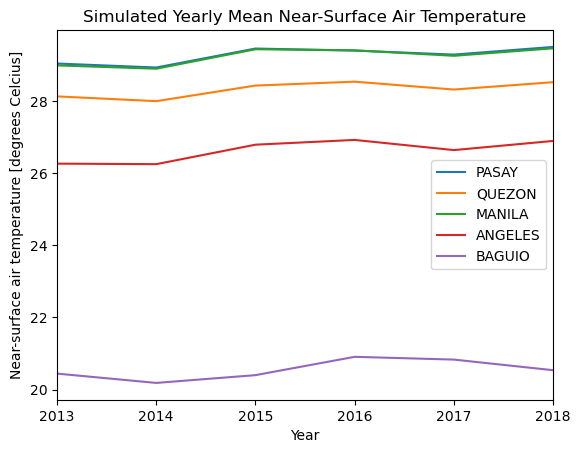
\includegraphics[width= 0.6 \textwidth]{hindcast/yearly-mean}
			\caption{
				The simulated yearly mean near-surface air temperature for each of the six cities (EIN15 ICBC with 8 km horizontal resolution).
			}
			\label{fig:hindcast-yearly-mean}
		\end{figure}

		For all cities, the year 2014 has the lowest yearly mean air temperature.
		The air temperature then rises for the years 2015 and 2016,
			lowers for the year 2017,
			before rising again in the year 2018,
				except for Baguio which lowers.
		One reason for this may be because of El Niño-Southern Oscillation effects.
		The years of El Niño-Southern Oscillation effects are as follows:
			2012 to 2013 and 2013 to 2014 correspond to a neutral year,
			2014 to 2015 corresponds to a weak El Niño,
			2015 to 2016 corresponds to a very strong El Niño,
			2016 to 2017 corresponds to a weak La Niña,
			and
			2017 to 2018 also corresponds to a weak La Niña
			(\cite{Null2025}).
		Since 2016 is a year of very strong El Niño effects, the mean temperature of that year is heightened for all cities analyzed.

		\begin{figure}	
			\centering
			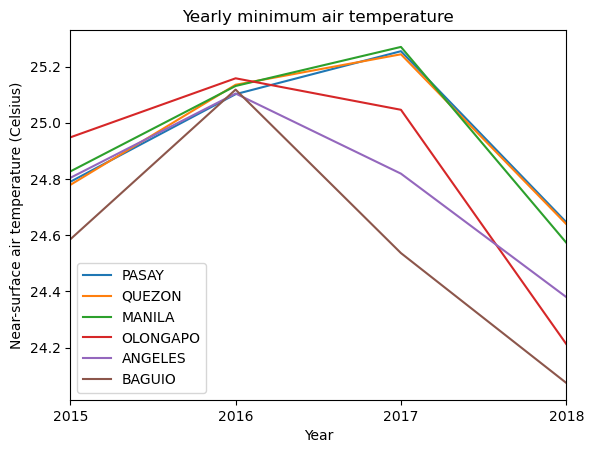
\includegraphics[width = 0.45\textwidth]{hindcast/yearly-min}
			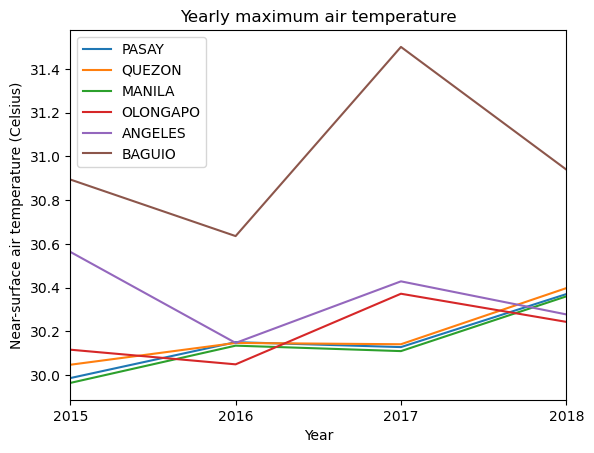
\includegraphics[width = 0.45\textwidth]{hindcast/yearly-max}
			\caption{
				The simulated yearly minimum and maximum near-surface air temperature for each of the six cities (EIN15 ICBC with 8 km horizontal resolution).
			}
			\label{fig:hindcast-yearly-min-max}
		\end{figure}
	
		Figure \ref{fig:hindcast-yearly-min-max} shows the yearly minimum and maximum near-surface air temperature for the cities.
		The maximum for all cities except Baguio can reach around $\qtyrange{37}{39}{\degreeCelsius}$ per year.
		Meanwhile, Baguio's maximum reaches around $\qty{29}{\degreeCelsius}$. 
			
		\begin{figure}	
			\centering
			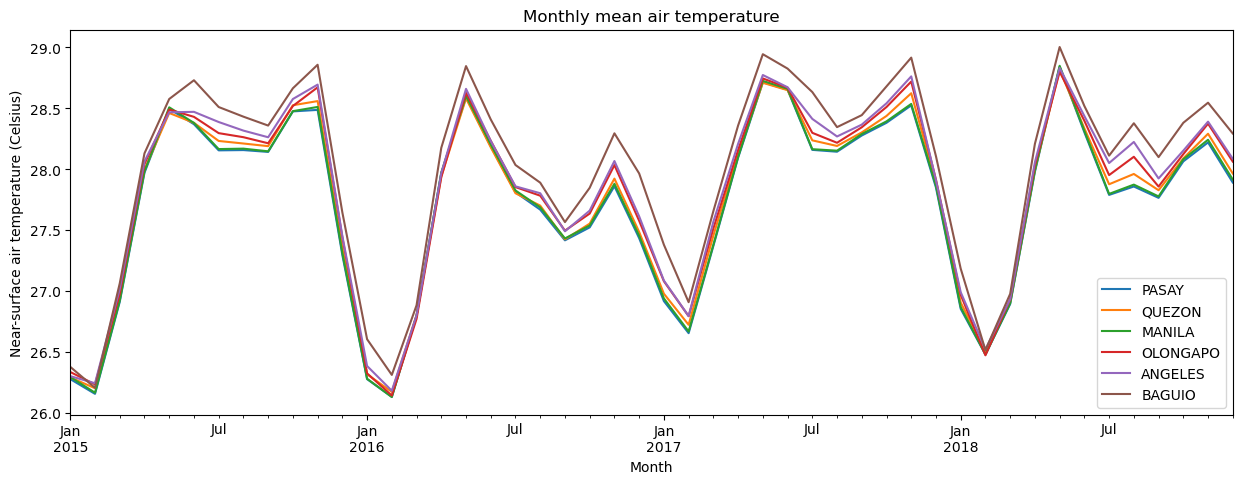
\includegraphics[width = \textwidth]{hindcast/monthly-mean}
			\caption{
				The simulated monthly mean near-surface air temperature for each of the six cities (EIN15 ICBC with 8 km horizontal resolution).
			}
			\label{fig:hindcast-monthly-mean}
		\end{figure}
	
		Figure \ref{fig:hindcast-monthly-mean} shows the simulated monthly mean near-surface air temperature.
		From the figure, February appears to be the coldest month per year.
		From then, air temperature rises until it peaks at May.
		Air temperature then lowers, during the months of July to September,
			and then rises again, peaking at November.
		It then lowers until February, and the cycle repeats for the next year.
		These results match the expected seasonal trends for air temperature in the Philippines.
		
		\begin{figure}	
			\centering
			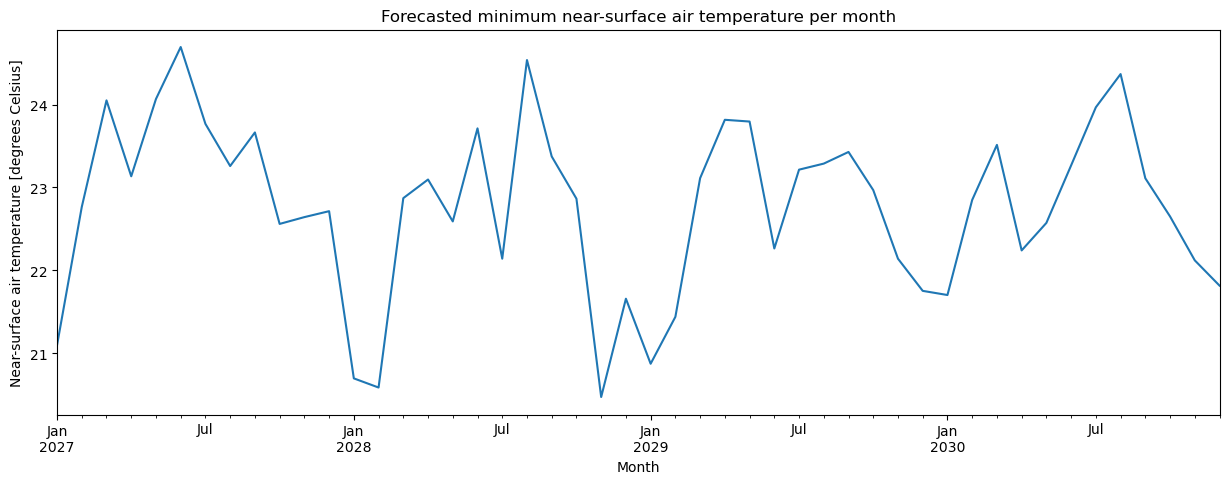
\includegraphics[width = \textwidth]{hindcast/monthly-min}
			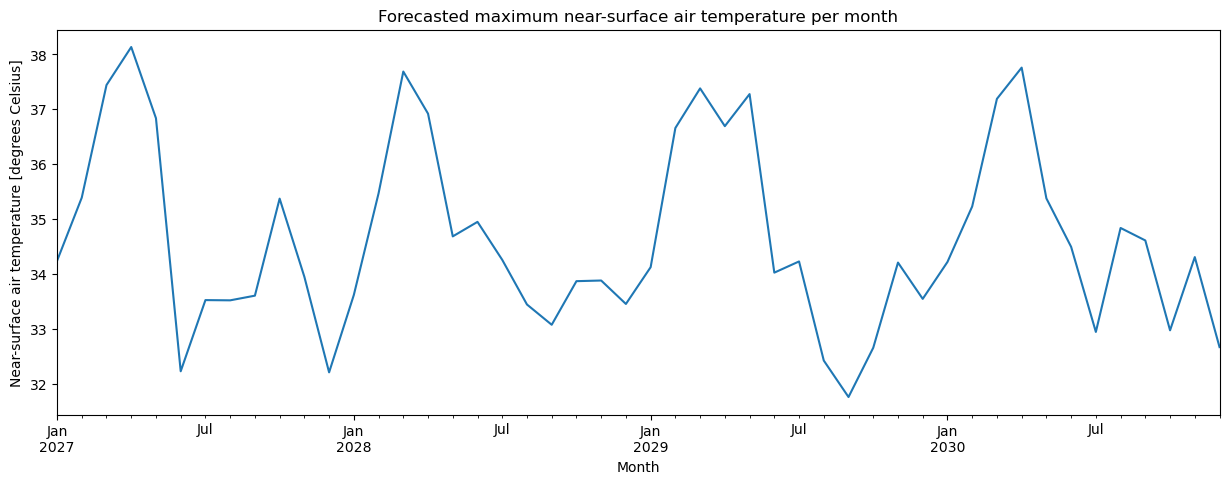
\includegraphics[width = \textwidth]{hindcast/monthly-max}
			\caption{
				The simulated monthly minimum and maximum near-surface air temperature for each of the six cities (EIN15 ICBC with 8 km horizontal resolution).
			}
			\label{fig:hindcast-monthly-min-max}
		\end{figure}

		\begin{figure}	
			\centering
			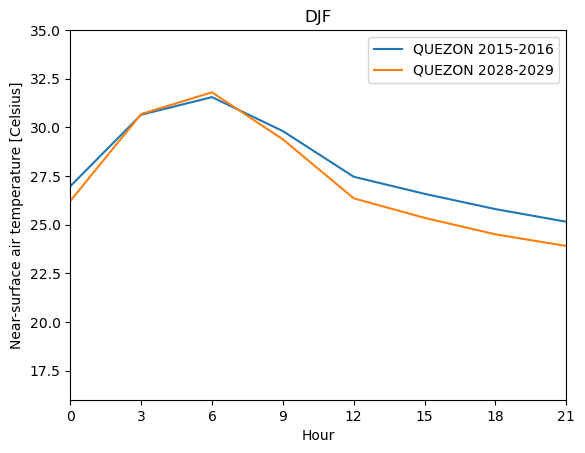
\includegraphics[width = 0.45 \textwidth]{hindcast/hourly-mean-djf}
			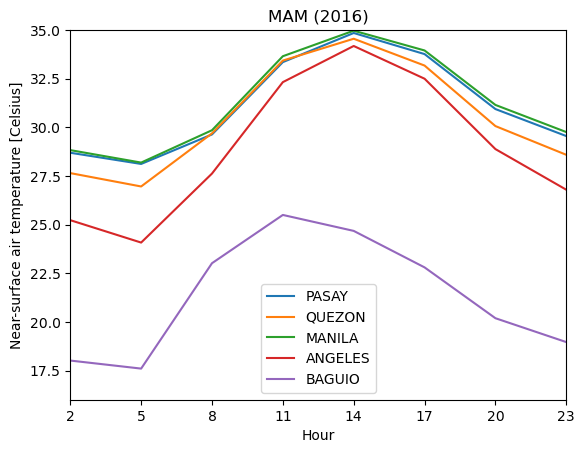
\includegraphics[width = 0.45 \textwidth]{hindcast/hourly-mean-mam}
			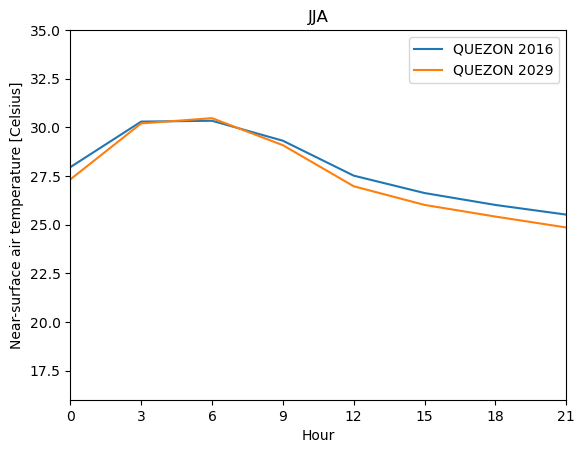
\includegraphics[width = 0.45 \textwidth]{hindcast/hourly-mean-jja}
			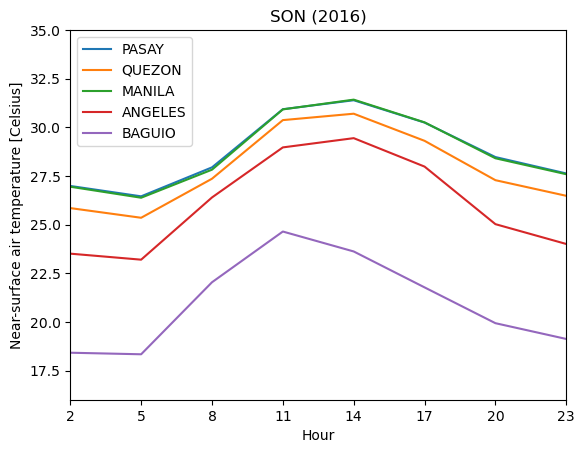
\includegraphics[width = 0.45 \textwidth]{hindcast/hourly-mean-son}
			\caption{
				Mean simulated near-surface air temperature each hour from 2015, December 1 to 2016, November 30, separated by three-month seasons (EIN15 ICBC with 8 km horizontal resolution).
				The seasons are:
					December, January, and February (DJF, upper left);
					March, April, and May (MAM, upper right);
					June, July, and August (JJA, lower left);
					and
					September, October, and November (SON, lower right).
			}
			\label{fig:hindcast-hourly-mean}
		\end{figure}
	
		Figure \ref{fig:hindcast-hourly-mean} shows the diurnal mean simulated near-surface air temperature from December 2015 to November 2016, split into three-month seasons:
			December, January, and February (DJF);
			March, April, and May (MAM);
			June, July, and August (JJA);
			and
			September, October, and November (SON).
		In all seasons, the mean air temperature is at its lowest at 9 PM, and peaks at 6 AM for all cities except Baguio, which peaks at 3 AM.
		The MAM season, corresponding to the Philippine's hot dry season, exhibits the highest air temperature compared to other seasons, in both daytime and nighttime.
		The JJA and SON seasons, which correspond to the Philippine wet season, show similar diurnal temperature patterns.
		The results for DJF, which correspond to the cool dry season, differ between cities.
		For the cities of Pasay, Quezon, and Manila, the DJF season has a similar pattern to JJA and SON.
		For the cities of Angeles and Baguio, the DJF season has cooler nighttime air temperature compared to JJA and SON, but have similar daytime air temperature.
		
		\begin{table}[]
			\caption{
				Mean simulated near-surface air temperature in degrees Celsius per season at 6 AM (Day), 6 PM (Night), and their difference (Diff.). Data simulated from December 2015 to November 2016.
			}
			\label{tab:hindcast-difference-day-night}
			\centering
			\begin{tabular}{lSSSSS}
				\hline \hline
				& {Pasay} & {Quezon} & {Manila} & {Angeles} & {Baguio} \\
				\hline
				      & \multicolumn{5}{c}{\textit{DJF}}           \\
				Day   & 32.0  & 31.6   & 32.2   & 30.5    & 23.4   \\
				Night & 27.2  & 25.8   & 27.1   & 22.9    & 16.7   \\
				Diff. & 4.8   & 5.8    & 5.1    & 7.6     & 6.7    \\
				& \multicolumn{5}{c}{\textit{MAM}}           \\
				Day   & 34.9  & 34.6   & 35.0   & 34.2    & 24.7   \\
				Night & 28.7  & 27.6   & 28.8   & 25.2    & 18.0   \\
				Diff. & 6.2   & 6.9    & 6.1    & 9.0     & 6.7    \\
				& \multicolumn{5}{c}{\textit{JJA}}           \\
				Day   & 31.3  & 30.3   & 31.1   & 29.7    & 22.8   \\
				Night & 27.3  & 26.0   & 27.3   & 24.2    & 19.1   \\
				Diff. & 3.9   & 4.3    & 3.8    & 5.4     & 3.7    \\
				& \multicolumn{5}{c}{\textit{SON}}           \\
				Day   & 31.4  & 30.7   & 31.4   & 29.4    & 23.6   \\
				Night & 27.0  & 25.9   & 26.9   & 23.5    & 18.4   \\
				Diff. & 4.4   & 4.9    & 4.5    & 5.9     & 5.2 \\
			  	\hline		
  			\end{tabular}
		\end{table}
		
		Table \ref{tab:hindcast-difference-day-night} shows the difference between daytime and noontime air temperature per season from December 2015 to November 2016.
		Since the diurnal air temperature peaks at 6 AM, this hour was chosen to represent daytime, while 6 PM is chosen to represent nighttime.
		The difference is greatest during the MAM season, and the least during JJA.
		Pasay and Manila have the least difference between day and night temperature,
			with a temperature of $\qty{3.9}{\degreeCelsius}$ and $\qty{3.8}{\degreeCelsius}$ during the JJA season,
			and a temperature of $\qty{6.2}{\degreeCelsius}$ and $\qty{6.1}{\degreeCelsius}$ during the MAM season,
			respectively.
		Meanwhile, Angeles shows the greatest difference, with a temperature of $\qty{5.4}{\degreeCelsius}$ during the JJA season, and $\qty{6.1}{\degreeCelsius}$ during the MAM season.
		These results may be explained by the relative urbanization of these cities.
		One characteristic of urban heat islands are high temperature at nighttime (\cite{Oke2017urban}).
		Pasay and Manila are the most urbanized among the cities, with little green spaces,
			and Quezon has relatively more green spaces compared to the other two cities (\cite{Bilang2022}).
		Furthermore, Angeles has vast green spaces surrounding it, which may explain the high difference between daytime and nighttime temperatures.
	
\section{Forecast}
	\subsection{SARIMA}
				
		\begin{figure}
			\centering
			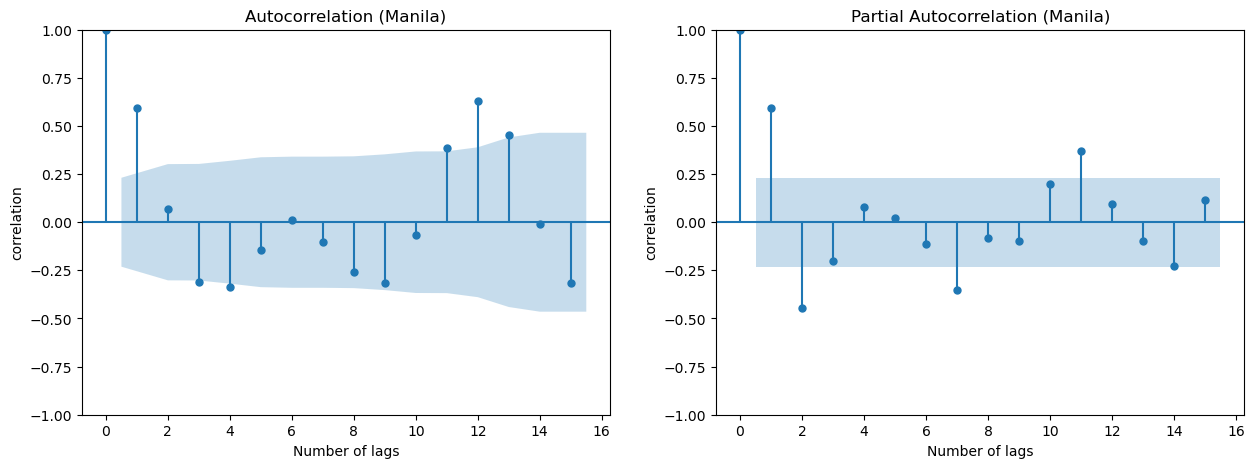
\includegraphics[width=\textwidth]{SARIMA/autocorrelations}
			\caption{
				Autocorrelation plots for the monthly mean time series data of Manila near-surface air temperature.
			}
			\label{fig:sarima-autocorrelations}
		\end{figure}	
		
		Figure \ref{fig:sarima-autocorrelations} shows the autocorrelation plots for Manila.
		For the autocorrelation plot, 
			there are significant negative correlations at $\num{3}$ and $\num4$ lags,
			suggesting that $p = 3$ and $p = 4$ are possible good values for the autoregressive factor.
		For the partial autocorrelation plot,
			there is a significant positive correlation at $\num{1}$ and $\num{2}$ lags,
			which suggest that $q = 1$ and $q = 2$ are possible good values for the moving average factor.
		
		\begin{table}[]
			\centering
			\caption{
				Evaluation results of various SARIMA parameters:
				Akaike information criterion (AIC),
				mean bias (MB),
				mean absolute error (MAE),
				and
				root mean square error (RMSE).
				Bolded parameters are best-performing out of all listed.
			}
			\label{tab:evaluation-sarima-parameters}
			\begin{tabular}{ccSSSS}
				\hline \hline
				{Order (p, d, q)} & {Seasonal Order (P, D, Q, S)} & {AIC}  & {MB}     & {MAE}   & {RMSE}  \\
				\hline
				(3, 1, 3)                           & None                                            & 126  & -0.938 & 1.00  & 1.24  \\
				(4, 1, 2)                           & None                                            & 130  & -0.217 & 0.800 & 1.07  \\
				(3, 1, 3)                           & (1, 1, 1, 12)                                   & 89.8 & -0.396 & 0.473 & 0.643 \\
				\textbf{(4, 1, 2)}                  & \textbf{(1, 1, 1, 12)}                          & 88.6 & -0.330 & 0.426 & 0.599 \\
				(3, 1, 3)                           & (1, 1, 0, 12)                                   & 89.5 & -0.383 & 0.520 & 0.680 \\
				(4, 1, 2)                           & (1, 1, 0, 12)                                   & 91.4 & -0.165 & 0.436 & 0.558 \\
				\hline			
			\end{tabular}
		\end{table}
	
		\begin{figure}
			\centering
			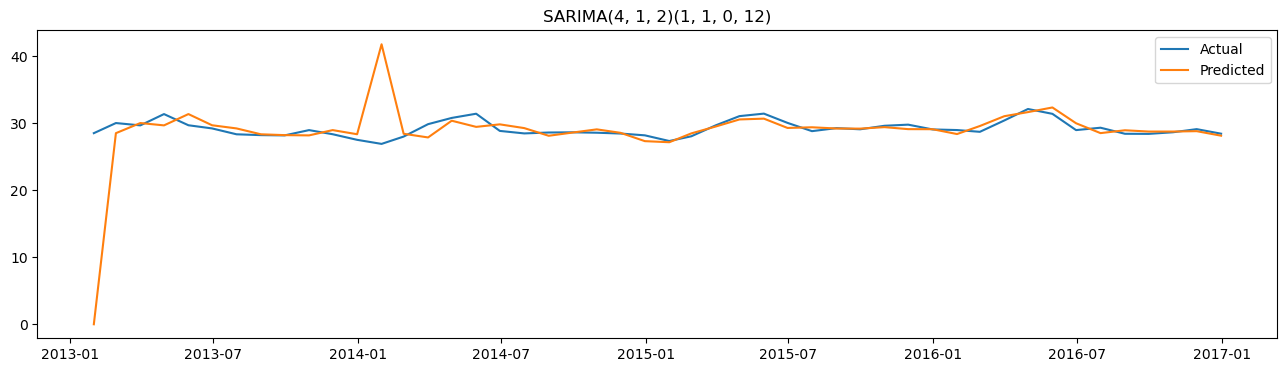
\includegraphics[width=\textwidth]{SARIMA/4 1 2 1 1 1 0 12 train}
			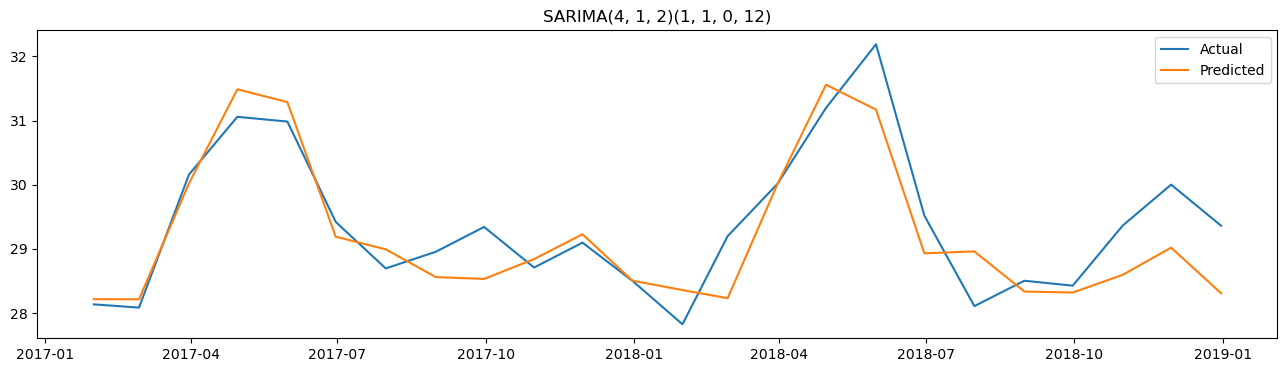
\includegraphics[width=\textwidth]{SARIMA/4 1 2 1 1 1 0 12 test}
			\caption{
				Graph of the best-performing model, $\operatorname{SARIMA}(4,1,2)(1,1,1,12)$, on training data (above) and testing data (below).
			}
			\label{fig:sarima-best-training-testing}
		\end{figure}
	
		Table \ref{tab:evaluation-sarima-parameters} shows the evaluation results of various SARIMA parameters.
		Models without a seasonal order show a higher AIC, MAE, and RMSE compared to models that do.
		Out of all tested models, the $\operatorname{SARIMA}(4,1,2)(1,1,1,12)$ model exhibits the least AIC, MAE, and RMSE values, which indicate that this is the best-performing model out of all the models tested. Figure \ref{fig:sarima-best-training-testing} shows a graph of this model over testing and training data.
		
		\begin{figure}
			\centering
			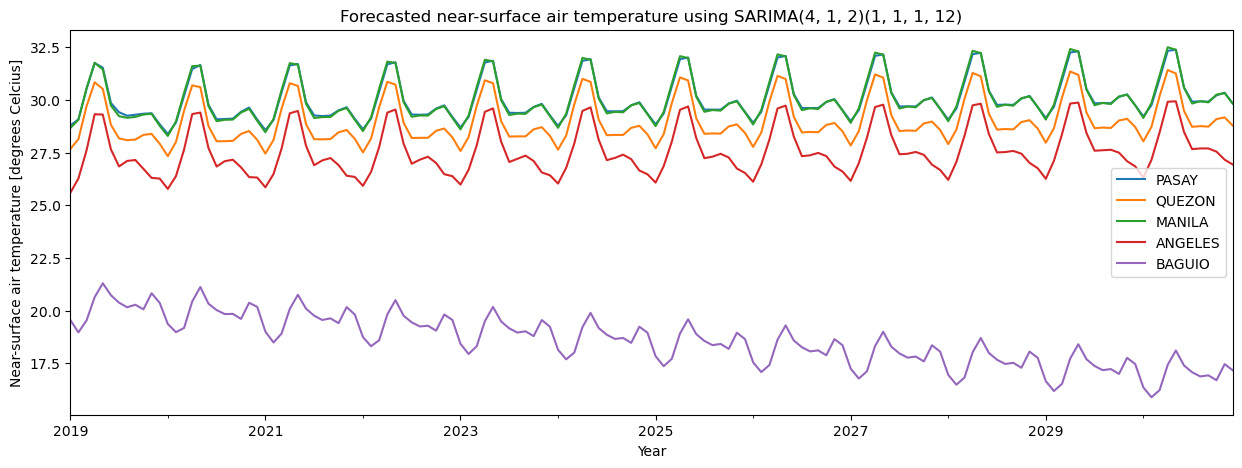
\includegraphics[width=\textwidth]{SARIMA/forecast}
			\caption{
				Forecast of near-surface air temperature in degrees Celsius using $\operatorname{SARIMA}(4,1,2)(1,1,1,12)$.
			}
			\label{fig:sarima-forecast}
		\end{figure}

\section{Limitations}
	One limitation of this study is that it only studies one variable, namely: near-surface air temperature.
	It does not examine ground temperature or temperature at different elevations.
	It also does not examine other factors that may be relevant to the study of urban heat islands, such as humidity, wind speed, wind direction, or precipitation. 
	Another limitation is that this study chose six specific cities to study: Angeles, Baguio, Manila, Olongapo, Pasay, and Quezon.
	Future studies may choose to study more cities.
	Another limitation is that this study only examines the three-year period from 2015 to 2017.
	Future studies may choose to study these other variables or study longer timeframes.
	
	There are many factors that can affect the findings. 
	Firstly, the physics schemes used in this run are all the default schemes, with the exception of the Community Land Model version 4.5 being chosen over the default BATS1e. 
	These runs do not use other models such as a lake model or a chemistry model, which may make the simulations more accurate and is an avenue for future research.
	Next, simulations are compared to the weather station data from the ISD.
	Only six stations were considered in this study.
	The data will be as accurate as the instruments used to record the data.
	Lastly, the study only used one domain.
	Changing the size and location of the domain without tweaking other settings can change the accuracy of the simulation.